
Figure \ref{fig:transformations} shows the transformation principle between the elements of the $\pi$-SCM meta-model used for representing the services' composition into the elements of the $\pi$-{\sc Pews} meta-model. There are two groups of rules: those that transform services' composition elements of the $\pi$-SCM to $\pi$-{\sc Pews} meta-models elements; and those that transform rules grouped by policies into {\em A-policy} types.

% _ . _ . _ . _ . _ . _ . _ . _ . _ . _ . _ . _ . _ . _ . _ . _ . _ . _ .
%\noindent

%{\bf\em 
\subsection{Transformation of the services' composition elements of the $\pi$-SCM to the $\pi$-{\sc Pews} elements}
% _ . _ . _ . _ . _ . _ . _ . _ . _ . _ . _ . _ . _ . _ . _ . _ . _ . _ .
A named action of the $\pi$-SCM represented by  {\sc\em Action} and {\sc\em Action:name} is transformed to a  named class {\sc Operation} with a corresponding attribute name {\sc Operation:name}. A  named service activity represented by the elements {\sc\em ServiceActivity}  and  {\sc\em ServiceActivity:name} of the $\pi$-SCM, are  transformed into a named operation of the $\pi$-{\sc Pews} represented by the elements  {\sc CompositeOperation} and {\sc CompositeOperation:name}. When more than one action is called, according to the following  composition patterns expressed using the operators {\sc\em merge, decision, fork and join} in the $\pi$-SCM the corresponding transformations, according to the PEWS operators presented above, are (see details in Figure \ref{fig:transformations}):
\begin{itemize}
\item   $op_1 . op_2$ if no {\sc\em ControlNode} is specified
\item ($op_1 \parallel op_2) . op_3$ if control nodes of type {\sc\em fork, join} are combined
 \item ($op_1 + op_2) . op_3$ if control nodes of type {\sc\em decision, merge} are combined
\end{itemize}

In the scenario "To Publish Music" the service activity {\sf PublishMusic} of the $\pi$-SC model specifies  calls to two {\sf Activitie}s of type {\em UpdateMusic}, respectively concerning the {\sf Business Service}s {\em Facebook} and {\em Twitter}. Given that no {\sf ConstrolNode} is specified by the $\pi$-SC model, the corresponding transformation is the expression that defines a {\sf Composite Operation} named {\em PublishSong} of the $\pi$-{\sc Pews} model of the form ({\sf PublishFacebook} $\parallel$ {\sf PublishTwitter}).
\begin{figure}
\centering{
%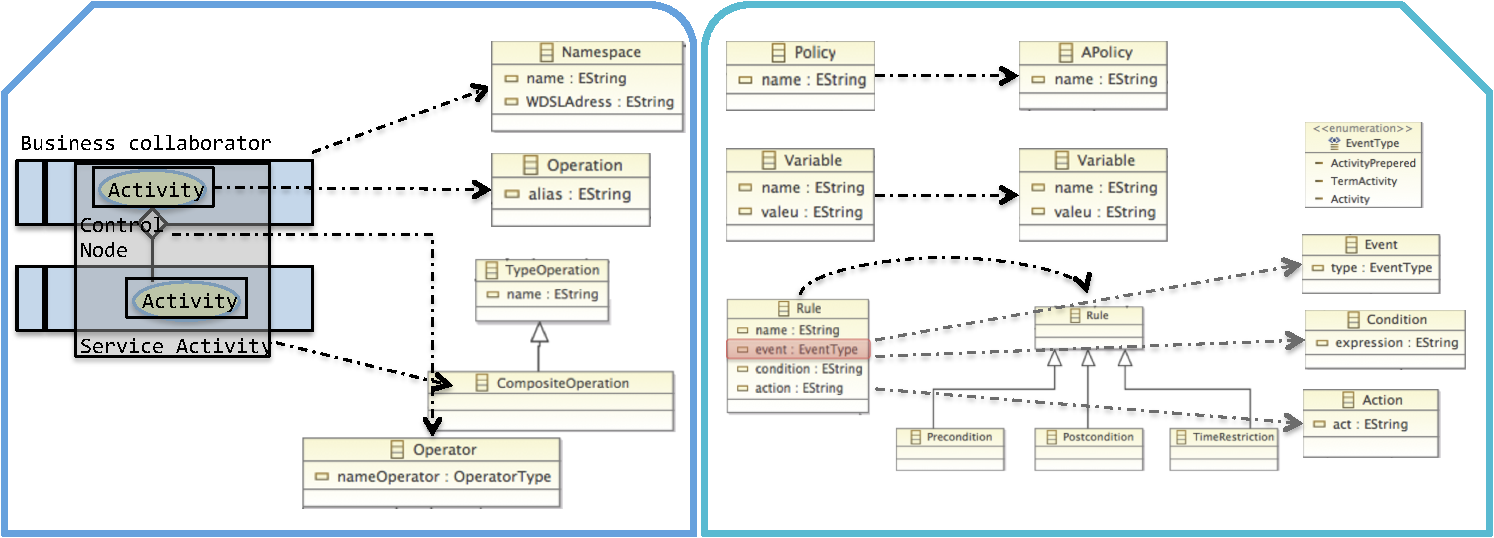
\includegraphics[width=0.80\textwidth]{figs/PI-SC-PI-P}}
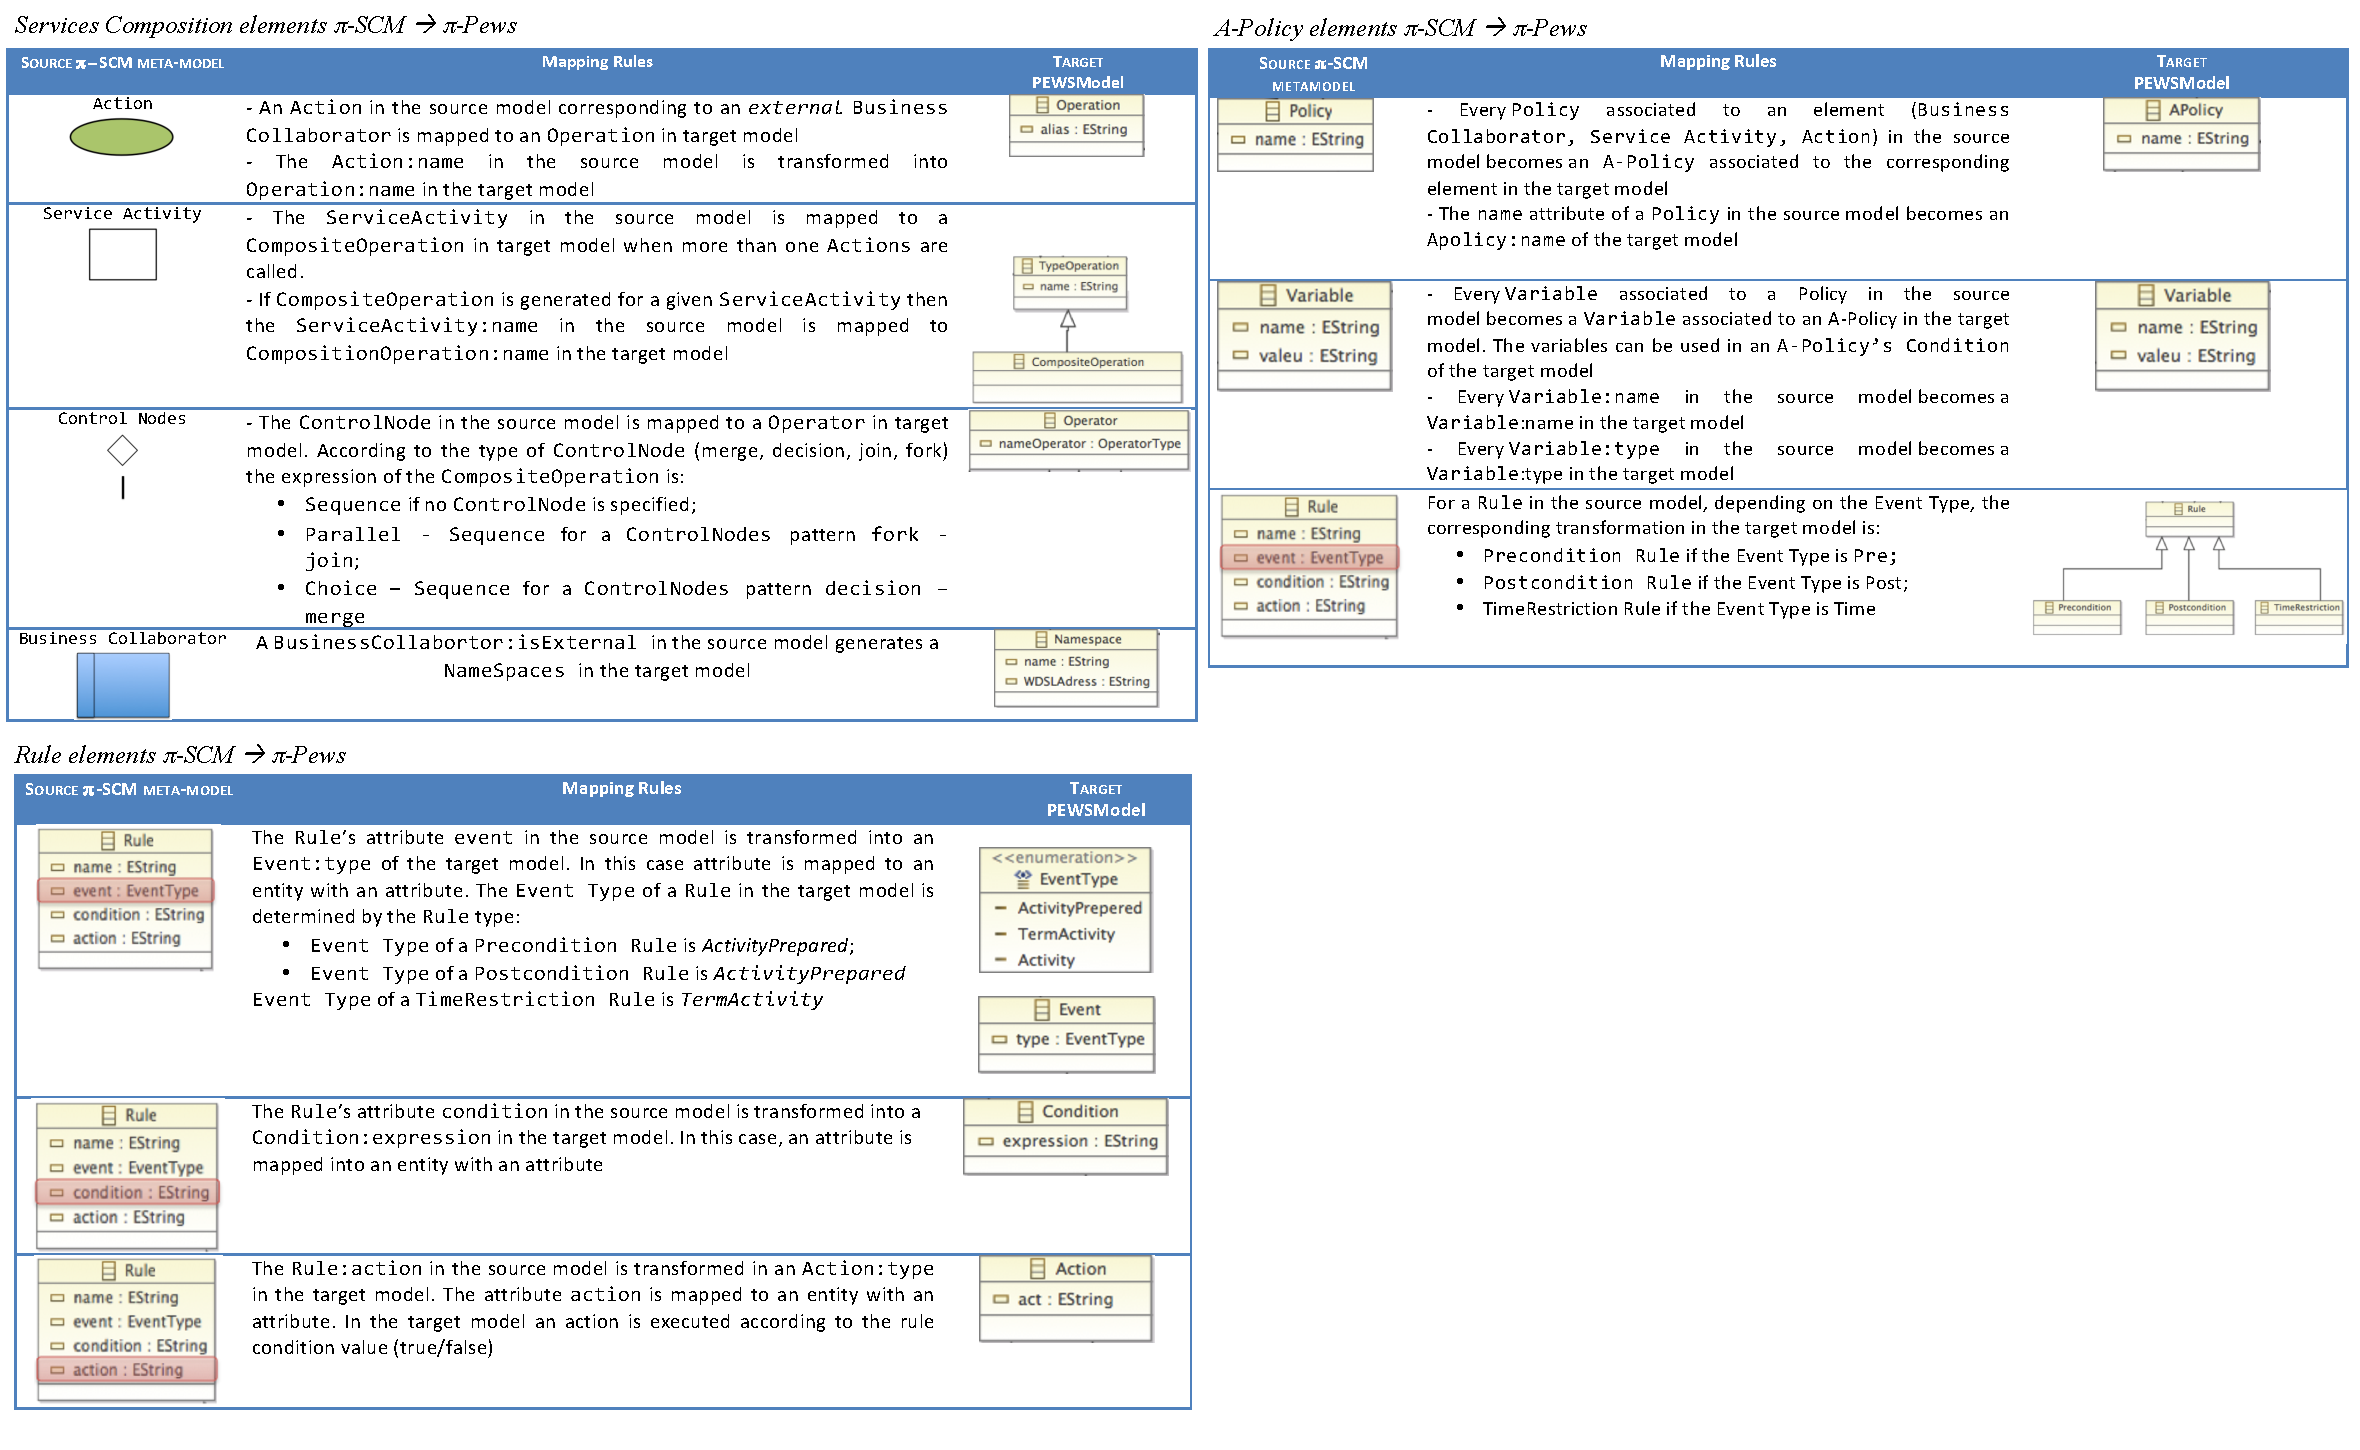
\includegraphics[width=0.96\textwidth]{figs/Mapping-1}}
\caption{ $\pi$-SCM to $\pi$-{\sc Pews} transformation}
\label{fig:transformations}
\end{figure}

% _ . _ . _ . _ . _ . _ . _ . _ . _ . _ . _ . _ . _ . _ . _ . _ . _ . _ .
%\noindent

%{\bf\em 
\subsection{Transformation of rules grouped by A-policies   in the $\pi$-SCM to A-Policies of  $\pi$-{\sc Pews}}
% _ . _ . _ . _ . _ . _ . _ . _ . _ . _ . _ . _ . _ . _ . _ . _ . _ . _ .
The {\em A-policies} defined for the elements of the $\pi$-SCM are transformed into {\sc A-Policy} classes, named according to the names expressed in the source model. The transformation of the rules expressed in the $\pi$-SCM is guided by the event types associated to these rules.   The variables associated to an {\em A-policy} expressed in the $\pi$-SCM as {\sc\em $<$Variable:name, Variable:type$>$} are transformed into elements of type {\sc Variable} with attributes {\sc name} and {\sc type} directly specified from the elements {\sc\em  Variable:name} and {\sc\em Variable:type} of the $\pi$-SCM model.

As shown in Figure \ref{fig:transformations}, for an event of type {\sc\em Pre} the corresponding transformed rule is of type {\sc Precondition}; for an event of type {\sc\em Post} the corresponding transformed rule is of type {\sc Postcondition}; finally, for an event of type {\sc\em TimeRestriction} the corresponding transformed rule is of type {\sc Time}. 
The condition expression of a rule in the $\pi$-SCM ({\sc\em Rule:condition}) is transformed into a class {\sc\em Condition:expression} where the attributes of the expression are transformed into elements of type {\sc Attribute}.

%The attribute event of a rule  ({\sc\em Rule:event}) in the $\pi$-SCM is transformed into an {\sc Event Type} according to the rule type. 

%As shown in Figure \ref{fig:transformations}, the event type for a rule of type (i) {\sc Precondition} is {\sc ActivityPrepared}; (ii) {\sc Postcondition} is {\sc TermActivity}; (iii) {\sc TimeRestriction} is {\sc Temporal}. The {\sc\em Rule:Action} of a rule in the $\pi$-SCM is transformed into an {\sc Action:type}.

%
%Figure \ref{fig:p-scim} shows the  $\pi$-{\sc Pews} model for our example.
In the scenario "To Publish Music" the {\sf Policies} {\em OAuthPolicy} and {\em HTTPAuthPolicy} of the $\pi$-SCM model are transformed into {\em A-policies} of type {\sf Precondition} of the $\pi$-{\sc Pews} model of the scenario. Thus in both cases the events are of type {\sf ActivityPrepared}. These policies, as stated in the $\pi$-SCM model, are associated to {\sf Activities}. In the corresponding transformation they are associated to {\sf Operation}s {\em PublishFacebook} and {\em PublishTwitter}.
%\begin{figure}[htpb]
%\centering{
%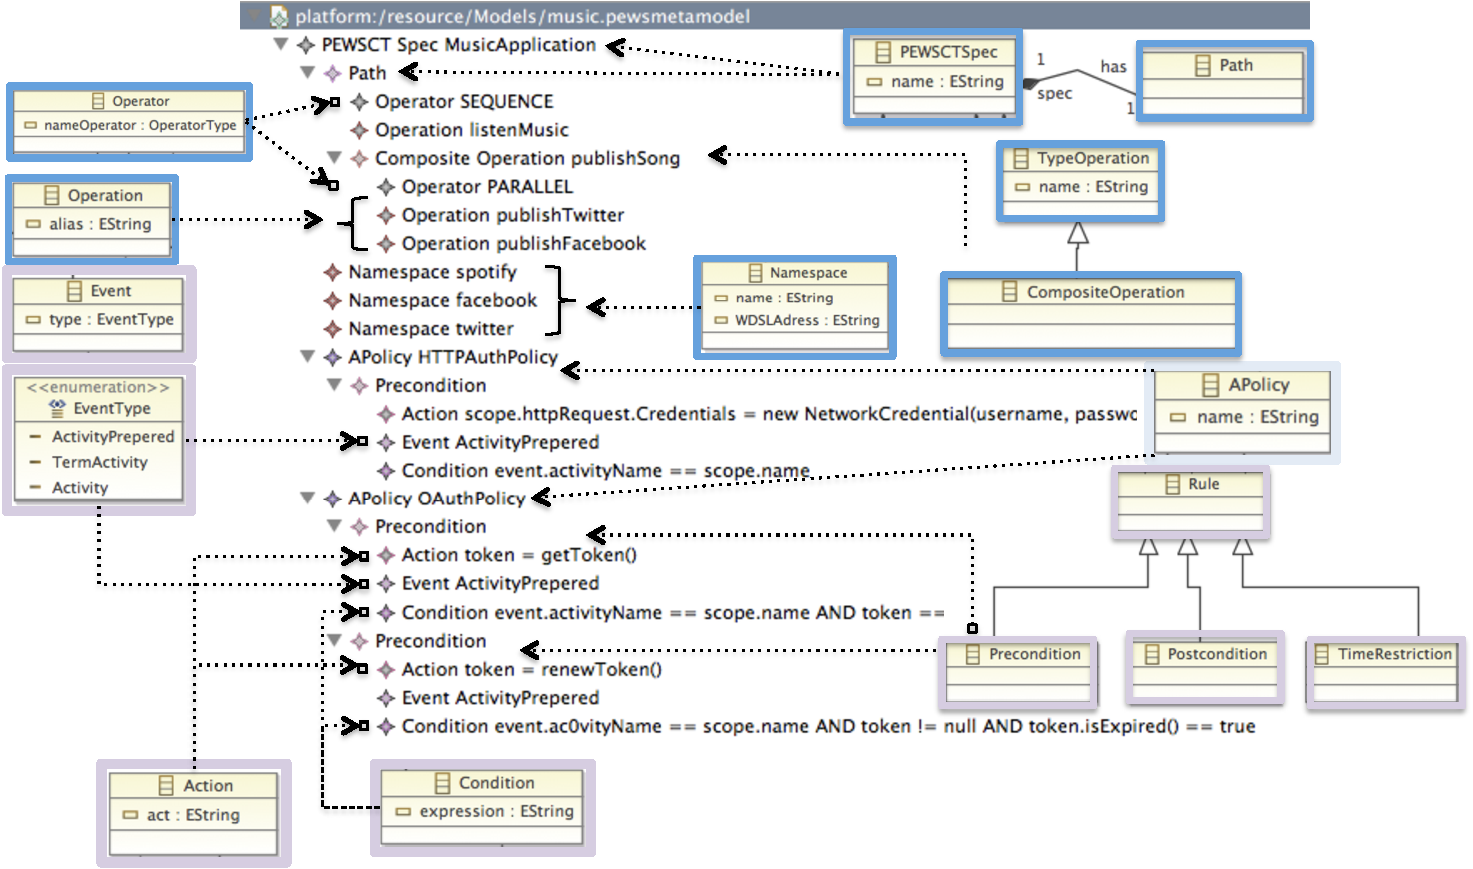
\includegraphics[width=0.78\textwidth]{figs/modeloPEWS}}
%\caption{$\pi$-{\sc Pews} generated model fo the "To Publish Music" application}
%\label{fig:p-scim}
%\end{figure}

%Figure \ref{fig:pewsexpression} shows the correspondence between the model and the statements that implement it, with a schematic representation of the business process.
%\begin{figure}
%\centering{
%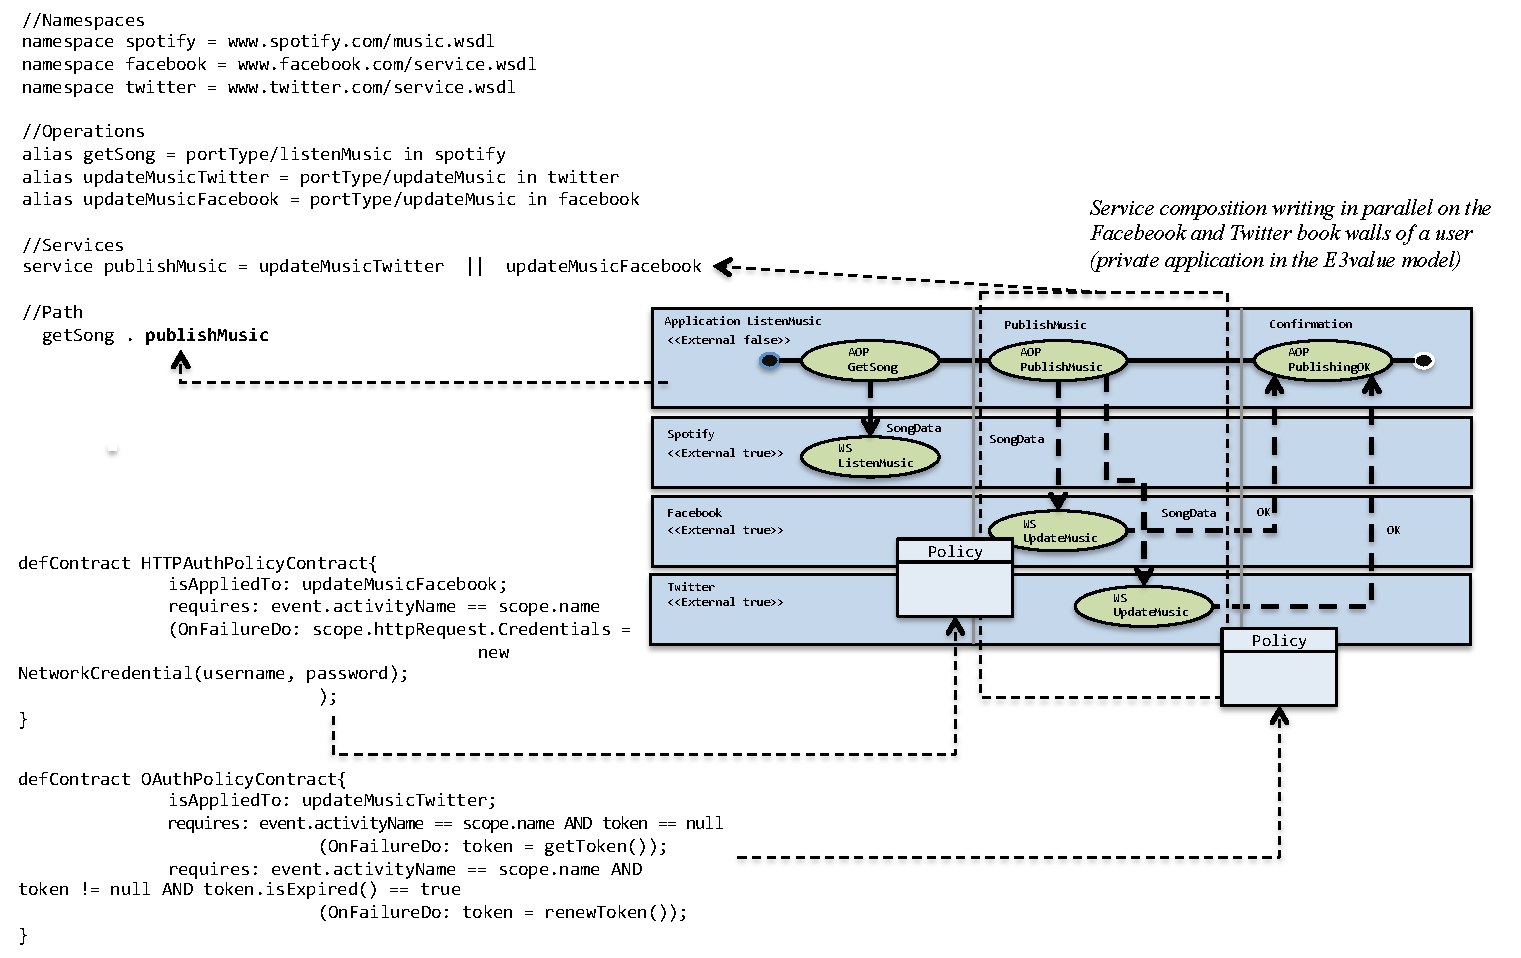
\includegraphics[width=0.85\textwidth]{figs/pews-expression}}
%\caption{Pews program implementing the "To Publish Music" application}
%\label{fig:pewsexpression}
%\end{figure}